\documentclass{beamer}

\usefonttheme[onlymath]{serif}
\usepackage[utf8]{inputenc}
\usepackage[english]{babel}
\usepackage{graphicx}
\usepackage{color}
\usepackage{natbib}
\usepackage{amsfonts}
\usepackage{amssymb}
\usepackage{amsmath}
\usepackage{amsthm}
\usepackage{bm}
\usepackage{algorithm}
\usepackage{algpseudocode}
\usepackage{caption}
\usepackage{tikz}
\usetikzlibrary{arrows,calc,tikzmark,shapes.misc}

\tikzset{every picture/.style=remember picture}
% Define a TikZ node for math content:
\newcommand{\mathnode}[2]{%
  \mathord{\tikz[baseline=(#1.base), inner sep = 0pt]{\node (#1) {$#2$};}}}

  \usetikzlibrary{shapes.arrows}
  \tikzset{MyArrow/.style={single arrow, draw, minimum width=10mm, minimum height=25mm,
                           inner sep=0mm, single arrow head extend=1mm}
  }



\DeclareMathOperator*{\argmin}{arg\,min}
\DeclareMathOperator*{\argmax}{arg\,max}

\newcommand{\gilles}[1]{\textcolor{red}{{\it GL: #1}}}

\newcommand{\bftheta}{{\bm \theta}}
\newcommand{\bfpsi}{{\bm \psi}}
\newcommand{\bfphi}{{\bm \phi}}
\newcommand{\bflambda}{{\bm \lambda}}
\newcommand{\bfx}{\mathbf{x}}
\newcommand{\bfz}{\mathbf{z}}


% Beamer layout
\hypersetup{colorlinks=True, citecolor=green, linkcolor=blue}

\let\oldbibitem=\bibitem
\renewcommand{\bibitem}[2][]{\label{#2}\oldbibitem[#1]{#2}}
\let\oldcite=\cite
\renewcommand\cite[1]{\hyperlink{#1}{\oldcite{#1}}}
\let\oldcitep=\citep
\renewcommand\citep[1]{\hyperlink{#1}{\oldcitep{#1}}}
\let\oldciteauthor=\citeauthor
\renewcommand\citeauthor[1]{\hyperlink{#1}{\oldciteauthor{#1}}}

\usetheme{boxes}
\beamertemplatenavigationsymbolsempty
\setbeamertemplate{sections/subsections in toc}[circle]
\setbeamertemplate{footline}[frame number]
\setbeamertemplate{itemize items}[circle]
\setbeamertemplate{itemize subitem}[square]

% Front slide
\title{{\bf Teaching machines to discover particles}}
\author{{Gilles Louppe}}
%\date{December 15, 2016}
\date{}

\tikzset{
  invisible/.style={opacity=0},
  visible on/.style={alt={#1{}{invisible}}},
  alt/.code args={<#1>#2#3}{%
    \alt<#1>{\pgfkeysalso{#2}}{\pgfkeysalso{#3}} % \pgfkeysalso doesn't change the path
  },
}

\begin{document}

\begin{frame}[plain]
\titlepage
\centering
\includegraphics[height=2.5em]{figures/nyu.jpg}
\end{frame}



% ==============================================================================

\begin{frame}
    \begin{center}
        \includegraphics[width=\textwidth]{figures/catchup.jpg}\\
        Catch-up session for Kyle's yersterday talk
    \end{center}
\end{frame}

\begin{frame}
    \centering {\bf \Large Background}
\end{frame}

\begin{frame}
    \frametitle{A few words about myself}

    {\it Background:}
    \begin{itemize}
        \item Training in computer science
        \item PhD in machine learning
            \begin{itemize}
                {\scriptsize \item  Contributions to random forests \\
                                    (interpretation, randomness, scalability, etc)}
            \end{itemize}
    \end{itemize}

    {\it Machine learning for Science:}
    \begin{itemize}
        \item As a PhD, I grew an interest for scientific applications of ML.
    \end{itemize}

    \vspace{0.5cm}

    \centering
    \begin{columns}
        \begin{column}{0.25\textwidth}
            \centering
            \includegraphics[width=\textwidth]{figures/cytomine.png}\\
            \scriptsize Recognition algorithms for biomedical images
        \end{column}
        \begin{column}{0.25\textwidth}
            \centering
            \includegraphics[width=\textwidth]{figures/connectomics.jpg}\\
            \scriptsize Connectome reconstruction algorithms
        \end{column}
        \begin{column}{0.25\textwidth}
            \centering
            \includegraphics[width=\textwidth]{figures/gwas.png}\\
            \scriptsize Genome-wide associations studies with ML
        \end{column}
    \end{columns}
\end{frame}



\begin{frame}
    \frametitle{Postdoc'ing at CERN + NYU}

    \begin{itemize}
        \item Joined CERN, and then NYU, as a postdoc with the goal of applying ML to particle physics data.

        \vspace{0.5cm}

        \item Switched gears in terms of research:
        \begin{itemize}
            {\scriptsize \item Contributions in likelihood-free inference, adversarial learning, domain adaptation, ...
                         \item Driven by particle physics applications.}
        \end{itemize}

        \vspace{0.5cm}

        \item Team work with physicists and researchers in ML.
        % show faces: kyle, kagan, lukas, tim, david, cho ...

        \begin{center}
            \includegraphics[width=0.125\textwidth]{figures/faces/kyle.png}\
            \includegraphics[width=0.125\textwidth]{figures/faces/lukas.png}\
            \includegraphics[width=0.125\textwidth]{figures/faces/juan.png}\
            \includegraphics[width=0.125\textwidth]{figures/faces/michael.png}

            \includegraphics[width=0.125\textwidth]{figures/faces/tim.png}\
            \includegraphics[width=0.125\textwidth]{figures/faces/cho.png}\
            \includegraphics[width=0.125\textwidth]{figures/faces/david.png}
        \end{center}
    \end{itemize}
\end{frame}


\begin{frame}
    \frametitle{Physics jargon vs. ML lingo}

    \begin{center}
        Physicists and machine learning researchers\\
        do not speak the same language.
    \end{center}

    \begin{columns}
        \begin{column}{0.4\textwidth}
            \centering
            \includegraphics[width=\textwidth]{figures/bb-hep.jpg}
        \end{column}
        \begin{column}{0.5\textwidth}
            \centering
            \includegraphics[width=\textwidth]{figures/bb-ml.jpg}
        \end{column}
    \end{columns}

    \vspace{0.5cm}


    {\scriptsize
    \begin{itemize}
        \item Due/thanks to its large collaborations, particle physics has often siloed itself and (re-)developed its own tools.
        \item This results in a barrier between physicists and outsiders, despite sometime using the same underlying concepts.
    \end{itemize}
    }

    \vspace{0.5cm}


    {\color{red}Disclaimer.} Ask if things are unclear!

    % disclaimer
    % interrupt if things are unclear
\end{frame}


% ==============================================================================

\begin{frame}
    \centering {\bf \Large Particle Physics 101}
\end{frame}

\begin{frame}
    \frametitle{The scientific method}

    \begin{center}
        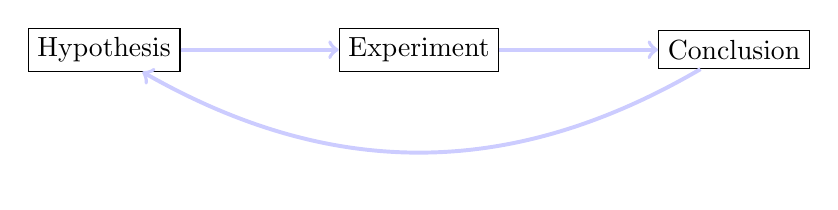
\begin{tikzpicture}
          \node[draw] (Hypothesis) at (0,0) {Hypothesis};
          \node[draw] (Experiment) at (4,0) {Experiment};
          \node[draw] (Conclusion) at (8,0) {Conclusion};

          \draw[->,draw=blue!20, line width=0.5mm] (Hypothesis) to (Experiment);
          \draw[->,draw=blue!20, line width=0.5mm] (Experiment) to (Conclusion);
          \draw[->,draw=blue!20, bend left, line width=0.5mm] (Conclusion) to (Hypothesis);
        \end{tikzpicture}
    \end{center}

    \vspace{-1cm}

    \begin{columns}[t]
        \begin{column}{0.23\textwidth}
            \centering
            \includegraphics[width=\textwidth]{figures/higgs.png}\\
            {\scriptsize The Higgs boson exists}
        \end{column}
        \begin{column}{0.23\textwidth}
            \centering
            \includegraphics[width=\textwidth]{figures/atlas.jpg}\\
            {\scriptsize LHC+ATLAS+CMS}
        \end{column}
        \begin{column}{0.23\textwidth}
            \centering
            \includegraphics[width=0.75\textwidth]{figures/discovery.png}\\
            {\scriptsize Discovery!}
        \end{column}
    \end{columns}

    \vspace{0.5cm}

    {\small

    \begin{itemize}
        \item The scientific method = recurrence over the sequence ``hypothesis, experiment and conclusion''.
        \item Conclusions are routinely automated through statistical inference, in which machine learning methods are embedded.
        \item Hypothesis and experiments are usually left for the scientists to decide.
    \end{itemize}}

    % illustrate each step with the particle physics correspondant
\end{frame}

\begin{frame}
    \frametitle{Testing for new physics}
    \vspace{0.5em}
    \only<1>{
    \begin{columns}
        \begin{column}{0.55\textwidth}
            \centering
            \includegraphics[width=\textwidth]{figures/phd1.png}
        \end{column}
        \begin{column}{0.4\textwidth}
            \centering
            \includegraphics[width=\textwidth]{figures/lhc1.jpg}\\
            \includegraphics[width=\textwidth]{figures/lhc2.jpg}\\
        \end{column}
    \end{columns}
    }
    %
    \only<2>{
    \begin{columns}
        \begin{column}{0.55\textwidth}
            \centering
            \includegraphics[width=\textwidth]{figures/phd2.png}
        \end{column}
        \begin{column}{0.4\textwidth}
            \centering
            \includegraphics[width=\textwidth]{figures/lhc3.jpg}
        \end{column}
    \end{columns}
    }
    %
    \only<3>{
    \begin{columns}
        \begin{column}{0.55\textwidth}
            \centering
            \includegraphics[width=\textwidth]{figures/phd3.png}\\

        \end{column}
        \begin{column}{0.4\textwidth}
            \hspace*{-0.5cm}
            \includegraphics[width=1.1\textwidth]{figures/plot-higgs.png}\\
            \centering
            \vspace{0.5cm}
            Hypothesis test based on the likelihood ratio
            $$\frac{p(\bfx | \text{background})}{p(\bfx | \text{background} + \text{signal})}$$
        \end{column}
    \end{columns}
    }
    \begin{tikzpicture}[remember picture,overlay]
        \node[left, yshift=-0.25cm] at (current page.north east) {\tiny Credits: Jorge Cham, \href{http://phdcomics.com/comics/archive.php?comicid=1489}{PHD comics}};
    \end{tikzpicture}
\end{frame}

\begin{frame}
    \frametitle{The Standard Model}

    \begin{center}
        \includegraphics[width=\textwidth]{figures/model.png}

        \vspace{0.5cm}
        The {\bf \color{red} uniqueness} of particle physics lies\\
         in its highly precise and compact model.
    \end{center}

    \begin{tikzpicture}[remember picture,overlay]
        \node[left, yshift=-0.25cm] at (current page.north east) {\tiny Credits: Kyle Cranmer};
    \end{tikzpicture}
\end{frame}


% ==============================================================================

\begin{frame}
    \centering {\bf \Large Machine learning $\cap$ Particle physics}
\end{frame}



\begin{frame}
    \frametitle{The players}

    \begin{columns}
        \begin{column}{0.35\textwidth}
            \centering
            {\Large $\bftheta := (\bm\mu, \bm\nu)$}\\
            Parameters

            \vspace{1cm}

            {\Large $\bm \mu$}\\
            Parameters of interest

            \vspace{1cm}

            {\Large $\bm \nu$}\\
            Nuisance parameters

            \vspace{1cm}

            {\Large $\bfz$}\\
            Latent variables
        \end{column}
        \begin{column}{0.4\textwidth}
            \centering

            Forward modeling\\
            Generation\\
            Simulation

            \vspace{0.25cm}

            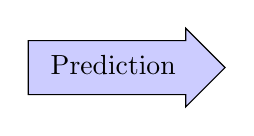
\begin{tikzpicture}
                \path (0,0) node[anchor=west,MyArrow,fill=blue!20] (a1) {\strut Prediction};
            \end{tikzpicture}

            \vspace{0.75cm}

            {\Huge $p(\bfx | \bftheta)$}

            \vspace{0.75cm}

            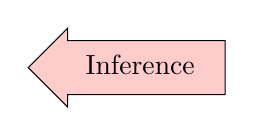
\begin{tikzpicture}
                \path (0,0) node[anchor=east,MyArrow,shape border rotate=180,fill=red!20] (a1) {\strut Inference};
            \end{tikzpicture}

            \vspace{0.25cm}

            Inverse problem\\
            Unfolding\\
            Measurement\\
            Parameter search

        \end{column}
        \begin{column}{0.35\textwidth}
            \centering

            {\Large $\bfx \sim p_r(\bfx)$}\\
            Observations drawn from Nature

            \vspace{1cm}

            {\Large $\bfx \sim p(\bfx|\bftheta)$}\\
            Simulated data \\
            (a lot!)
        \end{column}
    \end{columns}

    % illustrate several problems and relate to both ML and physics use cases
    % huge data
    % eg. terminology mismatch => explain terms in both physics and ML lingo
\end{frame}

\begin{frame}
    \frametitle{Likelihood-free assumptions}

    Operationally,
    $$\bfx \sim p(\bfx | \bftheta) \equiv \bfz \sim p(\bfz | \bftheta), \bfx = g(\bfz; \bftheta)$$
    where
    \begin{itemize}
        \item $\bfz$ provides a source of randomness;
        \item $g$ is a non-differentiable deterministic function (e.g. a computer program).
    \end{itemize}

    \vspace{0.5cm}

    Accordingly, the density $p(\bfx | \bftheta)$ can be written as
    $$p(\bfx | \bftheta) = \int_{\{ \bfz : g(\bfz; \theta) = \bfx \} } p(\bfz | \bftheta) \mu(d\bfz) $$

    \vspace{0.5cm}

    Evaluating the integral is often {\color{red} intractable}.
\end{frame}

\begin{frame}
    \begin{center}
        \includegraphics[width=\textwidth]{figures/cms.png}

        \vspace{0.5cm}

        Determining and evaluating all possible execution paths and all $\bfz$ that lead to the observation $\bfx$ is not tractable.\\

        {\scriptsize (And even less, normalizing that thing!)}
    \end{center}
\end{frame}

\begin{frame}
    \frametitle{Testing hypothesis
    (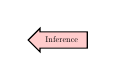
\begin{tikzpicture}[scale=0.3, every node/.style={scale=0.3,color=black}]
        \path (0,0) node[anchor=east,MyArrow,shape border rotate=180,fill=red!20] (a1) {\strut Inference};
    \end{tikzpicture})
    }

    Formally, physicists usually test a null $\bftheta = \bftheta_0$
     by constructing the likelihood ratio test
    statistic
    $$\Lambda({\cal D}; \bftheta_0) = \prod_{\bfx \in {\cal D}} \frac{p(\bfx | \bftheta_0)}{\sup_{\bftheta \in \bm\Theta} p(\bfx | \bftheta)} $$

    \begin{columns}
        \begin{column}{0.65\textwidth}
            \begin{itemize}
                \item Most measurements and searches for new particles are based on the distribution
                    of a single variable $\bfx \in \mathbb{R}$.

                \item The likelihood $p(\bfx | \bftheta)$ is approximated using 1D histograms.
                (Physicists love histograms!)

                \item Choosing a good variable $\bfx$ tailored for the goal of the experiment is the physicist's job.
            \end{itemize}
        \end{column}
        \begin{column}{0.34\textwidth}
            \begin{center}
                \includegraphics[width=\textwidth]{figures/histo.png}
            \end{center}
        \end{column}
    \end{columns}

\begin{center}
    {\it See Glen's talk today!}
\end{center}

\end{frame}

\begin{frame}
    \frametitle{Supervised learning
        (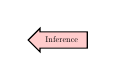
\begin{tikzpicture}[scale=0.3, every node/.style={scale=0.3,color=black}]
            \path (0,0) node[anchor=east,MyArrow,shape border rotate=180,fill=red!20] (a1) {\strut Inference};
        \end{tikzpicture})
    }

    {\it Setup:}
    \begin{itemize}
        \item Training data $\{ (\bfx_i, y_i) \in {\cal X} \times {\cal Y} | \bfx_i \sim p(\bfx | \bm \mu=y_i) \}_{i=1}^N$
        \item Learn a function $f : {\cal X} \to {\cal Y}$.
    \end{itemize}

    \vspace{0.5cm}

    \begin{columns}
        \begin{column}{0.7\textwidth}
            {\it In particle physics:}
            \begin{itemize}
                \item Part of a larger analysis
                \item To recognize signal from background events
                      and build a test statistic in the region of acceptance (e.g., ``cut-and-count'' analysis).
                \item To compress the data into a 1D value (more later).
            \end{itemize}
        \end{column}
        \begin{column}{0.3\textwidth}
            \begin{center}
                \includegraphics[width=\textwidth]{figures/cut.png}
            \end{center}
        \end{column}
    \end{columns}

    \begin{tikzpicture}[remember picture,overlay]
        \node[left, yshift=-0.25cm] at (current page.north east) {\tiny Credits: \href{https://arxiv.org/abs/1012.3589}{1012.3589}};
    \end{tikzpicture}
\end{frame}

\begin{frame}
    \frametitle{}
    \begin{itemize}
        \item Domain knowledge is traditionally incorporated as engineered features.

        \vspace{1cm}

        \item {\bf New paradigm:} Recent successes with deep learning models built on raw data is tickling physicists' curiosity.
            \begin{itemize}
                \item How to recast physics problems into well-studied ML problems?
                \item How to incorporate domain knowledge?
                \item Can we learn what these models have learned? ({\it See Daniel's talk tomorrow})
            \end{itemize}
    \end{itemize}
\end{frame}

\begin{frame}
    \frametitle{Particle physics detector as a camera}

    \begin{columns}
        \begin{column}{0.7\textwidth}
            \begin{center}
                \includegraphics[width=1.0\textwidth]{figures/sl-jets.png}
            \end{center}
        \end{column}
        \begin{column}{0.3\textwidth}
            \scriptsize
            Challenges:
            \begin{itemize}
                \item 3D volume of pixels
                \item Non-uniform geometry
                \item Mostly sparse
            \end{itemize}

            \begin{center}
                \includegraphics[width=0.8\textwidth]{figures/geometry.jpg}
            \end{center}
        \end{column}
    \end{columns}

    \begin{tikzpicture}[remember picture,overlay]
        \node[left, yshift=-0.25cm] at (current page.north east) {\tiny Images: \href{https://arxiv.org/abs/1612.01551}{1612.01551}};
    \end{tikzpicture}
\end{frame}

\begin{frame}
    \frametitle{Collision events as text paragraphs}

    \begin{columns}
        \begin{column}{0.65\textwidth}
            \begin{center}
                \includegraphics[width=0.9\textwidth]{figures/parse-tree.png}
            \end{center}

            {\scriptsize
            Analogy:
            \begin{itemize}
                \item word $\rightarrow$ particle
                \item sentence $\rightarrow$ jet
                \item parsing $\rightarrow$ jet algorithm
                \item paragraph $\rightarrow$ event
            \end{itemize}

            Domain knowledge is used to template the structure of the network, on a per-event basis.}
        \end{column}
        \begin{column}{0.3\textwidth}
            \centering
            \includegraphics[width=0.8\textwidth]{figures/qcd-rnn.png}\\
            \scriptsize \it QCD-aware recursive networks
        \end{column}
    \end{columns}

    \begin{tikzpicture}[remember picture,overlay]
        \node[left, yshift=-0.25cm] at (current page.north east) {\tiny Credits: \href{https://arxiv.org/abs/1702.00748}{1702.00748}};
    \end{tikzpicture}
\end{frame}

\begin{frame}
    \frametitle{Domain adaptation, Transfer learning
        (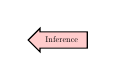
\begin{tikzpicture}[scale=0.3, every node/.style={scale=0.3,color=black}]
            \path (0,0) node[anchor=east,MyArrow,shape border rotate=180,fill=red!20] (a1) {\strut Inference};
        \end{tikzpicture})
    }

    {\it Setup:}
    \begin{itemize}
        \item Test data $\{ \bfx_i \sim p_r(\bfx) \}_{i=1}^N$
        \item $p_r(\bfx) \neq p(\bfx|\bftheta)$
    \end{itemize}

    \vspace{0.5cm}

    {\it In particle physics:}
    \begin{itemize}
        \item How does one build a model from simulated data that transfers well-enough to the true data distribution?
        \item How does one ensure the model does not exploit simulation artefacts?
    \end{itemize}

    \vfill
    \begin{center}
        \it Attend Michael's talk on Saturday!
    \end{center}
\end{frame}

\begin{frame}
    \frametitle{Learning under uncertainty
    (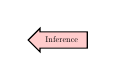
\begin{tikzpicture}[scale=0.3, every node/.style={scale=0.3,color=black}]
        \path (0,0) node[anchor=east,MyArrow,shape border rotate=180,fill=red!20] (a1) {\strut Inference};
    \end{tikzpicture})
    }

    \begin{itemize}
        \item Despite the precision of the SM, we still have to deal with:
            \begin{itemize}
                \item statistical uncertainties (inherent fluctuations)
                \item systematic uncertainties (the known unknowns of the model)
            \end{itemize}
        \item Uncertainty is usually formulated as nuisance parameters $\bm \nu$.
    \end{itemize}

    \vspace{0.1cm}

    \begin{columns}
        \begin{column}{0.5\textwidth}
            \centering
            \includegraphics[width=0.9\textwidth]{figures/pivot0.jpg}\\
            \includegraphics[width=0.9\textwidth]{figures/pivot1.jpg}\\
            \scriptsize \it With adversarial training, force the model to be independent of $\bm \nu$.
        \end{column}
        \begin{column}{0.5\textwidth}
            \centering
            \includegraphics[width=0.5\textwidth]{figures/param0.png}\\
            \includegraphics[width=0.6\textwidth]{figures/param1.png}\\
            \scriptsize \it Add $\bm \nu$ as an input to the model and profile it out later.
        \end{column}
    \end{columns}

    \begin{center}
        \it When to use one strategy  over the other?
    \end{center}
    \vspace{-1cm}

    \begin{tikzpicture}[remember picture,overlay]
        \node[left, yshift=-0.25cm] at (current page.north east) {\tiny Credits: \href{https://arxiv.org/abs/1611.01046}{1611.01046}, \href{https://arxiv.org/abs/1601.07913}{1601.07913}};
    \end{tikzpicture}
\end{frame}

\begin{frame}
    \frametitle{Likelihood-free inference
    (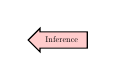
\begin{tikzpicture}[scale=0.3, every node/.style={scale=0.3,color=black}]
        \path (0,0) node[anchor=east,MyArrow,shape border rotate=180,fill=red!20] (a1) {\strut Inference};
    \end{tikzpicture})
    }

    Given observations $\bfx \sim p_r(\bfx)$, we seek: $$\bftheta^* = \arg \max_\theta p(\bfx | \bftheta)$$

    \begin{itemize}
        \item Histogramming $p(\bfx | \bftheta)$ does not scale to high dimensions.

        \item Can we automate or bypass the physicist's job of thinking about a good and compact representation for $\bfx$, without losing information?

        \item Hint: We do not need to know $p(\bfx|\bftheta)$ to find $\bftheta^*$.
    \end{itemize}

    % Likelihood-free: explain intractability
    % can generate data
    % insist on the assumptions
    % insist on the goal
    % hypothesis testing
    % carl as a generalization of histograms
    % profiling
\end{frame}

\begin{frame}
    \frametitle{Approximating likelihood ratios with classifiers}

The likelihood ratio $r(\bfx)$ is invariant under the change of variable $\bm u = s(\bfx)$, provided $s(\bfx)$ is monotonic with $r(\bfx)$:
$$r(\bfx) = \frac{p(\bfx|\bftheta_0)}{p(\bfx|\bftheta_1)} = \frac{p(s(\bfx)|\bftheta_0)}{p(s(\bfx)|\bftheta_1)} $$

A classifier $s$ trained to distinguish $\bfx \sim p(\bfx|\theta_0)$ from $\bfx \sim p(\bfx|\theta_1)$ satisfies the condition above.

\vspace{0.5cm}

This gives an automatic procedure for learning a good and compact representation for $\bfx$!

    \begin{tikzpicture}[remember picture,overlay]
        \node[left, yshift=-0.25cm] at (current page.north east) {\tiny Credits: \href{https://arxiv.org/abs/1506.02169}{1506.02169}};
    \end{tikzpicture}
\end{frame}

\begin{frame}

Therefore,
\begin{align*}
    \bftheta^* &= \arg \max_\theta p(\bfx | \bftheta) \\
               &= \arg \max_\theta \frac{p(\bfx | \bftheta)}{p(\bfx | \bftheta_1)} \\
               &= \arg \max_\theta \frac{p(s(\bfx;\bftheta,\bftheta_1) | \bftheta)}{p(s(\bfx;\bftheta,\bftheta_1) | \bftheta_1)}
\end{align*}
where $\bftheta_1$ is fixed and $s(\mathbf{x};\bftheta,\bftheta_1)$ is a family of classifiers trained to distinguish between $\bftheta$ and $\bftheta_1$.

    \begin{tikzpicture}[remember picture,overlay]
        \node[left, yshift=-0.25cm] at (current page.north east) {\tiny Credits: \href{https://arxiv.org/abs/1506.02169}{1506.02169}};
    \end{tikzpicture}
\end{frame}

\begin{frame}
    \frametitle{Learning in implicit generative models}

    Likelihood-free inference can be cast into the framework of ``implicit generative models''.

    \begin{columns}
        \begin{column}{0.35\textwidth}
            {\scriptsize
            This framework ties together:
            \begin{itemize}
                \item Approximate Bayesian computation
                \item Density estimation-by-comparison algorithms (two sample testing, density ratio, density difference estimation)
                \item Generative adversarial networks
                \item Variational inference
            \end{itemize}}
        \end{column}
        \begin{column}{0.65\textwidth}
            \begin{center}
                \includegraphics[width=\textwidth]{figures/implicit.png}
            \end{center}
        \end{column}
    \end{columns}

    \begin{tikzpicture}[remember picture,overlay]
        \node[left, yshift=-0.25cm] at (current page.north east) {\tiny Credits: \href{https://arxiv.org/abs/1610.03483}{1610.03483}};
    \end{tikzpicture}
\end{frame}

\begin{frame}
    \frametitle{}

    \begin{center}
        \includegraphics[width=0.7\textwidth]{figures/workshop.png}\\
        {\color{red} Hot topic in machine learning!}
    \end{center}
\end{frame}

% \begin{frame}
%     \frametitle{Probabilistic graphical models
%     (\begin{tikzpicture}[scale=0.3, every node/.style={scale=0.3,color=black}]
%         \path (0,0) node[anchor=east,MyArrow,shape border rotate=180,fill=red!20] (a1) {\strut Inference};
%     \end{tikzpicture})
%     }
%     % probabilistic ML
%     % for physicists: ML is not only about building classifiers
%
%     % common for ML, see VI tuto NIPS
%     % MLE vs Bayesian inference =>    bastillon of frequentism for physics
%     % box model
%     % make the assumptions explicit
% \end{frame}

\begin{frame}
    \frametitle{Fast simulation
    (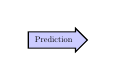
\begin{tikzpicture}[scale=0.3, every node/.style={scale=0.3,color=black}]
        \path (0,0) node[anchor=east,MyArrow,fill=blue!20] (a1) {\strut Prediction};
    \end{tikzpicture})
    }

    \begin{itemize}
        \item Half the LHC computing power (300000 cores) is dedicated to producing simulated data.
        \item Huge savings (in time and \$) if simulations can be made faster.
        \item Hand-made fast simulators are being developed by physicists, trading-off precision for speed.
    \end{itemize}

    \vfill
    \begin{center}
        \it Can we learn to generate data?\\
        (i.e. can we build a fast proxy for $\mathbf{x} \sim p(\bfx | \bftheta)$?)
    \end{center}

    % when to chose one or the other?
    % several layers of precision in simulation
    % fast simulations are useful
    % mention calogan & co
    % gans, vae, normalizing flows
\end{frame}

\begin{frame}
    \frametitle{Learning generative models
    (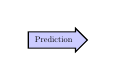
\begin{tikzpicture}[scale=0.3, every node/.style={scale=0.3,color=black}]
        \path (0,0) node[anchor=east,MyArrow,fill=blue!20] (a1) {\strut Prediction};
    \end{tikzpicture})
    }

    \begin{columns}
        \begin{column}{0.7\textwidth}
            \begin{center}
                \includegraphics[width=0.8\textwidth]{figures/lagan.png}\\
                \includegraphics[width=0.6\textwidth]{figures/calogan.png}
            \end{center}
        \end{column}
        \begin{column}{0.3\textwidth}
            \begin{center}
                \includegraphics[width=\textwidth]{figures/lagan2.png}
            \end{center}

            \scriptsize
            Challenges:
            \begin{itemize}
                \item How to ensure physical properties?
                \item Non-uniform geometry
                \item Mostly sparse
                \item GANs vs. VAE vs. Normalizing Flows?
            \end{itemize}
        \end{column}
    \end{columns}

    \begin{tikzpicture}[remember picture,overlay]
        \node[left, yshift=-0.25cm] at (current page.north east) {\tiny Credits: \href{https://arxiv.org/abs/1701.05927}{1701.05927}, \href{https://arxiv.org/abs/1705.02355}{1705.02355}};
    \end{tikzpicture}
\end{frame}

\begin{frame}
    \frametitle{How to evaluate generative models?}

    \begin{columns}
        \begin{column}{0.5\textwidth}
            \begin{center}
                \includegraphics[width=0.85\textwidth]{figures/calogan-plots.png}\\
                \scriptsize Physics: Evaluate well-known physical variates
            \end{center}
        \end{column}
        \begin{column}{0.5\textwidth}
            \begin{center}
                \includegraphics[width=0.95\textwidth]{figures/wgan.png}\\
                \scriptsize ML: Look at generated images
            \end{center}
        \end{column}
    \end{columns}

    \begin{center}
        {\color{red}This is not satisfying.} \\
        Can't we do better from a methodological standpoint?\\
        {\scriptsize (Some first steps at \href{https://arxiv.org/abs/1511.01844}{1511.01844})}
    \end{center}

    \begin{tikzpicture}[remember picture,overlay]
        \node[left, yshift=-0.25cm] at (current page.north east) {\tiny Credits: \href{https://arxiv.org/abs/1705.02355}{1705.02355}, \href{https://arxiv.org/abs/1704.00028}{1704.00028}};
    \end{tikzpicture}
\end{frame}


% ==============================================================================

\begin{frame}
    \centering {\bf \Large Outlooks} \\
    (a thought experiment)
\end{frame}

\begin{frame}
    \frametitle{Automating  the scientific process}
    \begin{center}
        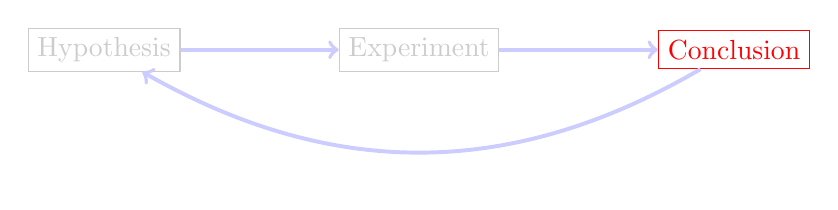
\begin{tikzpicture}
          \node[draw=black!20, color=black!20] (Hypothesis) at (0,0) {Hypothesis};
          \node[draw=black!20, color=black!20] (Experiment) at (4,0) {Experiment};
          \node[draw, color=red] (Conclusion) at (8,0) {Conclusion};

          \draw[->,draw=blue!20, line width=0.5mm] (Hypothesis) to (Experiment);
          \draw[->,draw=blue!20, line width=0.5mm] (Experiment) to (Conclusion);
          \draw[->,draw=blue!20, bend left, line width=0.5mm] (Conclusion) to (Hypothesis);
        \end{tikzpicture}
    \end{center}

    Most efforts are focused on automating the analysis of experimental results to draw conclusions,
    assuming the hypothesis and experiment are fixed.

    \begin{columns}
        \begin{column}{0.7\textwidth}
            \begin{center}
                \it Can we also automate \\
                    the steps of hypothesis and experiments?
            \end{center}
        \end{column}
        \begin{column}{0.25\textwidth}
            \begin{center}
                \includegraphics[width=\textwidth]{figures/cover.png}
            \end{center}
        \end{column}
    \end{columns}
\end{frame}

\begin{frame}
    \frametitle{Optimal experimental desgin}

    \begin{center}
        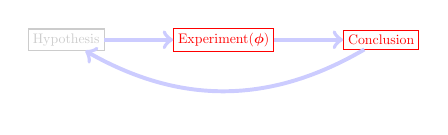
\begin{tikzpicture}[scale=0.5,every node/.style={scale=0.5}]
          \node[draw=black!20, color=black!20] (Hypothesis) at (0,0) {Hypothesis};
          \node[draw, color=red] (Experiment) at (4,0) {Experiment($\bm \phi$)};
          \node[draw, color=red] (Conclusion) at (8,0) {Conclusion};

          \draw[->,draw=blue!20, line width=0.5mm] (Hypothesis) to (Experiment);
          \draw[->,draw=blue!20, line width=0.5mm] (Experiment) to (Conclusion);
          \draw[->,draw=blue!20, bend left, line width=0.5mm] (Conclusion) to (Hypothesis);
        \end{tikzpicture}
    \end{center}

    Parameters $\bftheta$ of the (standard) model are known with uncertainty $H[\bftheta]$.
    {\it How to best reduce the uncertainty $H[\bftheta]$? }

    \begin{enumerate}
        \item Assume an experiment with parameters $\bm \phi$ can be simulated.
        \item Simulate the expected improvement $\Delta(\bm \phi) = H[\bftheta] - \mathbb{E}_{\text{data} | \bm \phi} [ H[\bftheta | \text{data} ] ]$.
            {\scriptsize
            \begin{itemize}
                \item This embeds the full likelihood-free inference procedure.
            \end{itemize}}
        \item Find $\bm \phi^* = \arg \max_{\bm \phi} \Delta(\bm \phi) $
            {\scriptsize
            \begin{itemize}
                \item Computationally (super) heavy.
            \end{itemize}}
    \end{enumerate}

    \vspace{0.5cm}

    {\scriptsize Connections to:
    \begin{itemize}
        \item Bayesian optimization
        \item Optimal experimental design
        \item Reinforcement learning (for a sequence of experiments)
    \end{itemize}}

\end{frame}

\begin{frame}
    \frametitle{Active sciencing}

    \onslide<1->{
    \begin{center}
        \includegraphics[width=\textwidth]{figures/flowchart.png}
    \end{center}
    }
    \onslide<2>{
    \begin{center}
        \includegraphics[width=0.75\textwidth]{figures/danilo.png}
    \end{center}
    }

    \begin{tikzpicture}[remember picture,overlay]
        \node[left, yshift=-0.25cm] at (current page.north east) {\tiny Credits: \href{https://github.com/cranmer/active_sciencing}{cranmer/active\_sciencing}};
    \end{tikzpicture}

\end{frame}

\begin{frame}
    \frametitle{Exploring the theory space}

    \begin{center}
        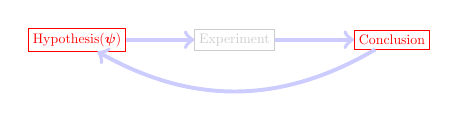
\begin{tikzpicture}[scale=0.5,every node/.style={scale=0.5}]
          \node[draw, color=red] (Hypothesis) at (0,0) {Hypothesis($\bm \psi$)};
          \node[draw=black!20, color=black!20] (Experiment) at (4,0) {Experiment};
          \node[draw, color=red] (Conclusion) at (8,0) {Conclusion};

          \draw[->,draw=blue!20, line width=0.5mm] (Hypothesis) to (Experiment);
          \draw[->,draw=blue!20, line width=0.5mm] (Experiment) to (Conclusion);
          \draw[->,draw=blue!20, bend left, line width=0.5mm] (Conclusion) to (Hypothesis);
        \end{tikzpicture}
    \end{center}

    \begin{columns}
        \begin{column}{0.7\textwidth}
            The Standard model admits several extensions.

            \vspace{0.5cm}

            {\it Can we explore the space of theories and find the envelope that agree with the data? }

            \begin{itemize}
                \item Assume a generative model of theories, indexed by $\bm \psi$.
                \item Assume the experiment design $\bm \phi$ is fixed.
                \item Find $\{ \bm \psi | \rho(p_r(\bfx | \bm \phi), p(\bfx|\bm \psi, \bm \phi, \bftheta^*)) < \epsilon \}$.
            \end{itemize}
        \end{column}
        \begin{column}{0.3\textwidth}
            \begin{center}
                \includegraphics[width=\textwidth]{figures/level.png}\\
                \includegraphics[width=\textwidth]{figures/auto2.png}
            \end{center}
        \end{column}
    \end{columns}
\end{frame}

\begin{frame}
    \frametitle{AI recipe for understanding Nature}

    \begin{center}
        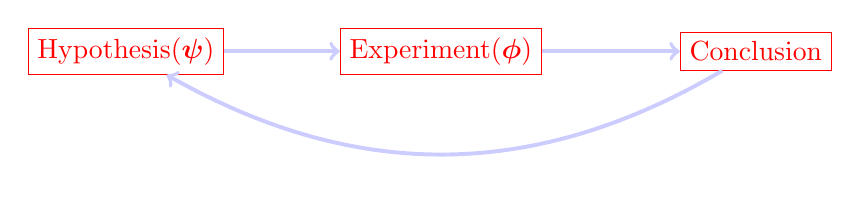
\begin{tikzpicture}
          \node[draw, color=red] (Hypothesis) at (0,0) {Hypothesis($\bm \psi$)};
          \node[draw, color=red] (Experiment) at (4,0) {Experiment($\bm \phi$)};
          \node[draw, color=red] (Conclusion) at (8,0) {Conclusion};

          \draw[->,draw=blue!20, line width=0.5mm] (Hypothesis) to (Experiment);
          \draw[->,draw=blue!20, line width=0.5mm] (Experiment) to (Conclusion);
          \draw[->,draw=blue!20, bend left, line width=0.5mm] (Conclusion) to (Hypothesis);
        \end{tikzpicture}
    \end{center}

    $$\text{Find}\, \{ \bm \psi | \rho(p_r(\bfx | \bm \phi), p(\bfx|\bm \psi, \bm \phi, \bftheta^*)) < \epsilon, \forall \bm \phi \}$$
\end{frame}


% ==============================================================================

\begin{frame}
    \centering {\bf \Large Summary}
\end{frame}

\begin{frame}
    \frametitle{Why collaborating with physicists?}

    \begin{itemize}
        \item Contribute to the understanding of the Universe.

        \vspace{1cm}

        \item Open methodological challenges.

        \vspace{1cm}

        \item Test bed for developing ambitious ML/AI methods, as enabled by the precise mechanistic understanding of physical processes.

        \vspace{1cm}

        \item Core problems in particle physics transfer to other fields of science (likelihood-free inference, domain adaptation, optimization, etc).
    \end{itemize}
\end{frame}

\end{document}
